
%-------------------------------------------
\documentclass{beamer}
\usepackage[utf8]{inputenc}
\usepackage{utopia} %font utopia imported
%-------------------------------------------------
% slide appearance
\usetheme{Boadilla}
\usecolortheme{default}

%-------------------------------------------------
% listing
\usepackage{listings}
\usepackage{xcolor}
\definecolor{codegreen}{rgb}{0,0.6,0}
\definecolor{codegray}{rgb}{0.5,0.5,0.5}
\definecolor{codepurple}{rgb}{0.58,0,0.82}
\definecolor{backcolour}{rgb}{0.95,0.95,0.92}
\lstdefinestyle{mystyle}{
    backgroundcolor=\color{backcolour},   
    commentstyle=\color{codegreen},
    keywordstyle=\color{magenta},
    numberstyle=\tiny\color{codegray},
    stringstyle=\color{codepurple},
    basicstyle=\ttfamily\footnotesize,
    breakatwhitespace=false,         
    breaklines=true,                 
    captionpos=b,                    
    keepspaces=true,                 
    numbers=left,                    
    numbersep=5pt,                  
    showspaces=false,                
    showstringspaces=false,
    showtabs=false,                  
    tabsize=2
}
\lstset{style=mystyle}
%--------------------------------------------------

% aide LaTeX : http://l.roussarie.free.fr/IMG/pdf/ltx101-4-2.pdf

\newcommand\FAIRB{FAIR{\_}bioinfo}

%------------------------------------------------------------
%This block of code defines the information to appear in the
%Title page
\title[FAIR{\_}Bioinfo] %optional
{FAIR{\_}bioinfo for bioinformaticians}

\subtitle{Introduction to the tools of reproducibility in bioinformatics}

\author[Céline, Thomas, Claire] % (optional)
{C.~Hernandez\inst{1} \and T.~Denecker\inst{1} \and  J.~Sellier\inst{2} \and G.~Le Corguillé\inst{2} \and C.~Toffano-Nioche\inst{1}}

\institute[I2BC-IFB] % (optional)
{
  \inst{1}%https://fr.overleaf.com/project/5e749e3c458ed8000166a12b
  Institute for Integrative Biology of the Cell (I2BC)\\
  UMR 9198, Université Paris-Sud, CNRS, CEA\\
  91190 - Gif-sur-Yvette, France
\and
  \inst{2}%
  IFB Core Cluster taskforce
}

\date[IFB 2020] % (optional)
{Sept. 2020}
\logo{
\includegraphics[height=0.5cm]{shared/logo-ifb.jpg}}

%End of title page configuration block
%------------------------------------------------------------

%------------------------------------------------------------
%logos definition
 \newcommand{\logoAws}{\protect
\includegraphics[height=1.7ex,keepaspectratio]{shared/logo-aws.png}}
\newcommand{\logoCmake}{\protect
\includegraphics[height=1.7ex,keepaspectratio]{shared/logo-cmake.png}}
\newcommand{\logoCNRS}{\protect
\includegraphics[height=1.7ex,keepaspectratio]{shared/logo-CNRS.png}}
\newcommand{\logoConda}{\protect
\includegraphics[height=1.7ex,keepaspectratio]{shared/logo-conda.png}}
\newcommand{\logoDockerPaysage}{\protect
\includegraphics[height=1.7ex,keepaspectratio]{shared/logo-docker-paysage.png}}
\newcommand{\logoDockerPortrait}{\protect
\includegraphics[height=1.7ex,keepaspectratio]{shared/logo-docker-portrait.png}}
\newcommand{\logoDockerHub}{\protect
\includegraphics[height=1.7ex,keepaspectratio]{shared/logo-dockerHub.png}}
\newcommand{\logoGit}{\protect
\includegraphics[height=1.7ex,keepaspectratio]{shared/logo-git.png}}
\newcommand{\logoGithub}{\protect
\includegraphics[height=1.7ex,keepaspectratio]{shared/logo-github.png}}
\newcommand{\logoGoogleCloud}{\protect
\includegraphics[height=1.7ex,keepaspectratio]{shared/logo-googleClooud.png}}
\newcommand{\logoIdeuxBC}{\protect
\includegraphics[height=1.7ex,keepaspectratio]{shared/logo-i2bc.png}}
\newcommand{\logoIFB}{\protect
\includegraphics[height=1.7ex,keepaspectratio]{shared/logo-ifb.jpg}}
\newcommand{\logoJupyter}{\protect
\includegraphics[height=1.7ex,keepaspectratio]{shared/logo-jupyter.png}}
\newcommand{\logoMicrosoftAzure}{\protect
\includegraphics[height=1.7ex,keepaspectratio]{shared/logo-microsoftAzure.png}}
\newcommand{\logoNextflow}{\protect
\includegraphics[height=1.7ex,keepaspectratio]{shared/logo-nextflow.png}}
\newcommand{\logoRmarkdown}{\protect
\includegraphics[height=1.7ex,keepaspectratio]{shared/logo-Rmarkdown.png}}
\newcommand{\logoShiny}{\protect
\includegraphics[height=1.7ex,keepaspectratio]{shared/logo-shiny.png}}
\newcommand{\logoSingularity}{\protect
\includegraphics[height=1.7ex,keepaspectratio]{shared/logo-singularity.png}}
\newcommand{\logoSlurm}{\protect
\includegraphics[height=1.7ex,keepaspectratio]{shared/logo-slurm.png}}
\newcommand{\logoSnakemake}{\protect
\includegraphics[height=1.7ex,keepaspectratio]{shared/logo-snakemake.png}}
\newcommand{\logoVirtualbox}{\protect
\includegraphics[height=1.7ex,keepaspectratio]{shared/logo-virtualbox.png}}
\newcommand{\logoZenodo}{\protect
\includegraphics[height=1.7ex,keepaspectratio]{shared/logo-zenodo.png}}




\begin{document}

\frame{\titlepage}

\begin{frame}{Schedule}
%-------------------------------------------
Introduction to snakemake workflow\\
\quad \quad \textcolor{gray}{\it Exercise 1: one unique step}\\
From bash script to snakemake\\
\quad \quad \textcolor{gray}{\it Exercise 2: workflow of the RNAseq analysis}\\
\quad \quad \textcolor{gray}{\it Exercise 3: Running the snakemake workflow on our laptop}\\
\end{frame}

%-------------------------------------------
\subsection[WorkflowIntro]{Introduction to workflow}
%-------------------------------------------
\begin{frame}{}
    \huge{Introduction to snakemake workflow}
\end{frame}
%-------------------------------------------
\begin{frame}{Workflow definition}
%-------------------------------------------
\begin{block}{Linked commands}
 a pool of commands, progressively linked by the treatments of the input data towards the results:\\
    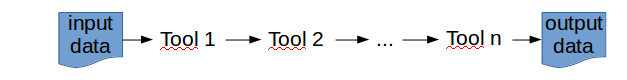
\includegraphics[width=12cm]{03_workflow/images/FAIR_workflow_schema.png}\\
   arrow: output of tool $n-1$ = input for tool $n$
\end{block}
\begin{block}{Data parallelization}
     several data flows can be processed in parallel 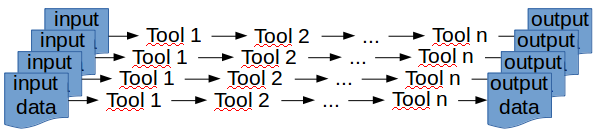
\includegraphics[width=12cm]{03_workflow/images/FAIR_workflow_schema_parallelization.png}
\end{block}
\end{frame}
%-------------------------------------------
\begin{frame}{A workflow is launched. How to reduce the waiting time?}
%-------------------------------------------
    Improve algorithms? Are we ready to optimize Bowtie2? hem ... no!\\
    We have multiple data and steps of analyses $\Rightarrow$ we can parallelize!\\
    \begin{center}
            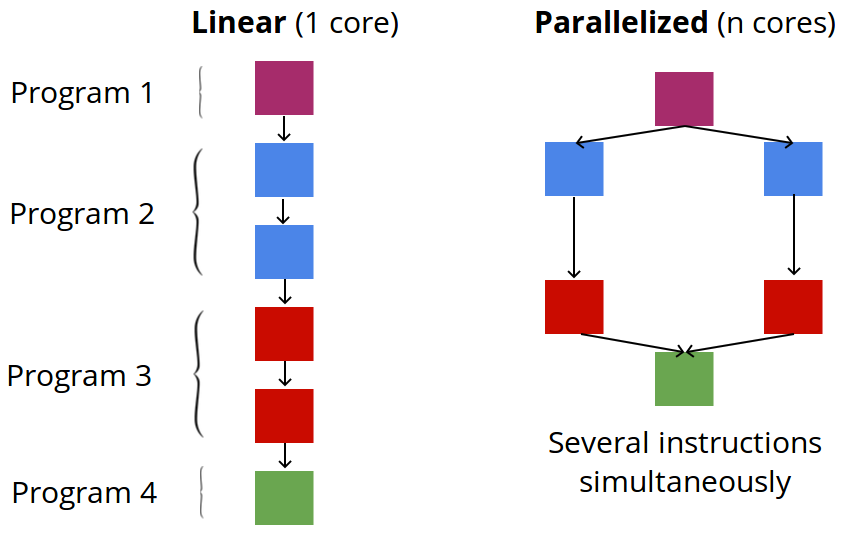
\includegraphics[height=6cm]{03_workflow/images/FAIR_WF_linear_vs_parallel_en.png}
    \end{center}
\end{frame}
%-------------------------------------------
\begin{frame}{Workflow management system}
%-------------------------------------------
Many workflow management systems, many forms:
\begin{itemize}
    \item command line: shell (but doesn't handle parallelization alone, need to script it, not easy)
    \item rule: 
\includegraphics[height=1cm]{shared/logo-snakemake.png}, 
\includegraphics[height=0.5cm]{shared/logo-cmake.png}, \logoNextflow, ...
    \item graphic interface: Galaxy, Taverna, Keppler, ...
\end{itemize}
\vfill
pros: important for reproducibility (keep track of when each file was generated, and by which operation), manage parallelization\\
cons: learning effort
\vfill
We choose 
\includegraphics[height=1cm]{shared/logo-snakemake.png}
\end{frame}
%-------------------------------------------
\begin{frame}[containsverbatim]
\frametitle{Snakemake rule}
%-------------------------------------------
Snakemake: mix of the programming language Python (snake) and the rule-based automation tool Make\footnote{Make: https://www.gnu.org/software/make/manual/}\\
Good practice: one step, one rule
\begin{block}{A rule is defined by it name and may contain:}
\begin{itemize}
    \item \verb|input:| list one or more file names
    \item \verb|output:| list one or more file names
    \item command (\verb|run:| for python ; \verb|shell:| for shell, R, etc)
\end{itemize}
+ optional directives: \verb|params:|, \verb|message:|, \verb|log:|, ...\\
Remark: with 1 command line, use a \verb|shell:| directive ; with many command lines, use a \verb|run:| directive with python shell("...") functions.
\end{block}
\begin{center}
    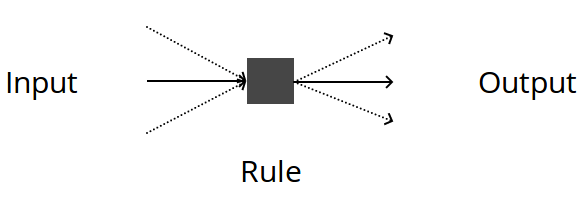
\includegraphics[height=1.8cm]{03_workflow/images/FAIR_WF_rule_concept_en.png}
\end{center}
\end{frame}
%-------------------------------------------
\begin{frame}[containsverbatim]
\frametitle{Hello World example}
%-------------------------------------------
The objective of this example is to write "Hello World" into the file \verb|world.txt| in the directory \verb|hello|:
\begin{block}{hello$\_$world.smk:}
\begin{lstlisting}
rule hello_world:
    output: "hello/world.txt"
    shell: "echo Hello World > hello/world.txt"
\end{lstlisting}
 % docker run -v ${PWD}:/home -w /home snakemake/snakemake snakemake -j1 --snakefile helloworld.smk 
\end{block}
\begin{itemize}
    \item the rule contains only an \verb|output:| directive (due to the usage of the \verb|echo| command)
\end{itemize}
\end{frame}
%-------------------------------------------
\begin{frame}{Snakemake}
%-------------------------------------------
Snakemake automatically makes sure that everything is up to date, otherwise it launch the jobs that need to be.
\vfill
Snakemake:
\begin{itemize}
    \item works on files (rather than streams, reading/writing from databases or passing variables in memory)
    \item is based on Python (but know how to code in Python is not required to work with Snakemake)
    \item has features for defining the environment with which each task is carried out (running a large number of small third-party tools is current in bioinformatics)
    \item is easily to be scaled from desktop to server, cluster, grid or cloud environments (ie. develop on laptop using a small subset of data, run the real analysis on a cluster)
\end{itemize}    
\end{frame}
%-------------------------------------------
\begin{frame}{Data flow linkage}
%-------------------------------------------
A snakemake workflow links rules thank to the filenames of the rule input and output directives:
\begin{center}
    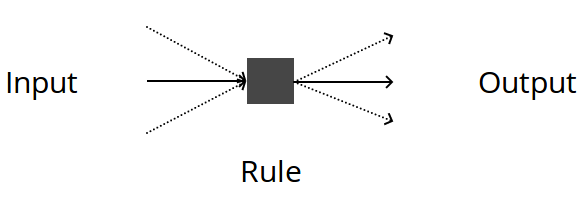
\includegraphics[height=1.8cm]{03_workflow/images/FAIR_WF_rule_concept_en.png}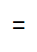
\includegraphics[height=1.8cm]{03_workflow/images/FAIR_signeEgal.png}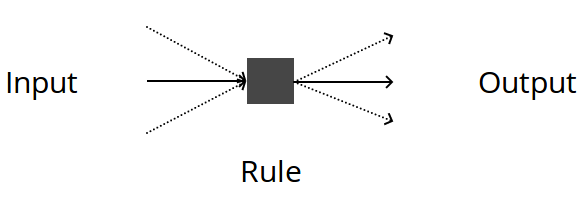
\includegraphics[height=1.8cm]{03_workflow/images/FAIR_WF_rule_concept_en.png}
\end{center}
\begin{block}{Snakemake rules order:}
   the first rule (all, target, ...) specifies the result files, the next rules describe how to achieve them.
\end{block}
\end{frame}
%-------------------------------------------
\begin{frame}[containsverbatim]
\frametitle{Rule execution order}
%-------------------------------------------
Snakemake starts with the first rule that describes the workflow result files. Since they do not exist, it "goes back" through the workflow until it finds an input file to apply a rule to. 
\begin{center}
    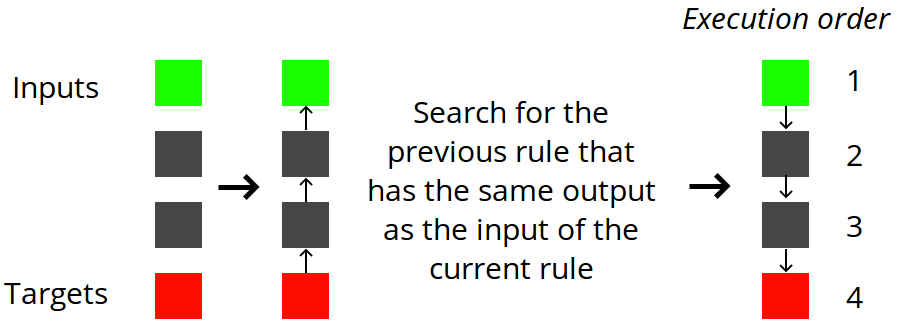
\includegraphics[height=3cm]{03_workflow/images/FAIR_smke_rule_order_en.png}
\end{center}
For determining whether output files have to be re-created, Snakemake checks whether the file modification date (i.e. the timestamp) of any input file of the job is newer than the timestamp of the output file.
\end{frame}
%-------------------------------------------
\begin{frame}[containsverbatim]
\frametitle{Generalization with wilcards}
%-------------------------------------------
Wildcards (Snakemake key feature) allow to replace hardcoded filenames and make input and output directives flexible. Using them will:
\begin{itemize}
\item reduce the amount of code needed
\item have the workflow work on new data, without modification
\end{itemize}
\vfill
In the filename, wildcards (writing into \verb|{}|) are automatically resolved (replaced by regular expression \verb|".+"|). All filenames matching the expression are concerning by the directive.
%write \verb|{wildcard_name}| in \verb|input:| or \verb|output:| directives and \verb|{wildcards.wildcard_name}| elsewhere.
Wildcards are specific to the rule, a same file can be accessed by different matching. :
\begin{block}{Ex. with the file "101$/$file.A.txt"}
\begin{lstlisting}
rule one: output: "{set}1/file.{grp}.txt" => set=10, grp=A
rule two: output: "{set}/file.A.{ext}" => set=101, ext=txt
\end{lstlisting}
\end{block}
\vfill
(more on \href{https://snakemake.readthedocs.io/en/stable/snakefiles/rules.html#wildcards}{\textcolor{blue}{\underline{wildcards}}} in the snakemake documentation)
\end{frame}
%-------------------------------------------
\begin{frame}[containsverbatim]
\frametitle{With and without wilcards examples}
%-------------------------------------------
\begin{block}{without$\_$wildcards$\_$uniprot.smk}
\begin{lstlisting}
rule all:
 input: "P10415.fasta", "P01308.fasta"

rule get_prot:
 output: "P10415.fasta", "P01308.fasta"
 run:
  shell("wget https://www.uniprot.org/uniprot/P10415.fasta")
  shell("wget https://www.uniprot.org/uniprot/P01308.fasta")
\end{lstlisting}
\end{block}
% bel exemple issu de https://endrebak.gitbooks.io/the-snakemake-book
% mais ping n'étant pas présent par défaut dans le docker snakemake 
% => remplacement par uniprot
%rule all:
%  input: "ping/github.txt", "ping/duckduckgo.txt"
%rule ping:
% output: "ping/github.txt", "ping/duckduckgo.txt
% run:
%  shell("ping -c3 github.com > ping/github.txt")
%  shell("ping -c3 duckduckgo.com > ping/duckduckgo.txt")
%
%rule ping:
% output: "ping/{host}.txt"
% run:
%  shell("ping -c3 {wildcards.host}.com > ping/{wildcards.host}.txt")
\begin{block}{with$\_$wildcards$\_$uniprot.smk}
\begin{lstlisting}
rule get_prot:
  output: "{prot}.fasta"
  run:
    shell("wget https://www.uniprot.org/uniprot/{wildcards.prot}.fasta")
\end{lstlisting}
\end{block}
\end{frame}
%-------------------------------------------
\begin{frame}[containsverbatim]
\frametitle{Input (output) specifications}
%-------------------------------------------
\begin{block}{enumerated}
\begin{lstlisting}
rule one:
  input: "P10415.fasta", "P01308.fasta"
\end{lstlisting}
\end{block}
\begin{block}{python list $\&$ wildcards}
\begin{lstlisting}
DATASETS = ["P10415", "P01308"]
rule one: 
  input: ["{dataset}.fasta".format(dataset=dataset) 
          for dataset in DATASETS] 
\end{lstlisting}
\end{block}
\begin{block}{expand() $\&$ wildcards}
\begin{lstlisting}
DATASETS = ["P10415", "P01308"]
rule one: 
  input: expand("{dataset}.fasta", dataset=DATASETS) 
\end{lstlisting}
\end{block}
\end{frame}
%-------------------------------------------
\begin{frame}[containsverbatim]
\frametitle{Snakemake acces}
%-------------------------------------------
\begin{block}{Laptop with docker}
\begin{lstlisting}[language=bash]
docker pull snakemake/snakemake  #install (linux: add sudo)
docker run -v ${PWD}:/data -w /data snakemake/snakemake snakemake ...  #run
\end{lstlisting}
\end{block}
\begin{block}{Laptop with conda}
\begin{lstlisting}[language=bash]
conda create -n smk-env -c bioconda snakemake  #install
conda activate smk-env ; snakemake ...         #run
\end{lstlisting}
\end{block}
\begin{block}{IFB core cluster}
\begin{lstlisting}[language=bash]
module load snakemake ; snakemake ...           #run
\end{lstlisting}
\end{block}
check access by replacing \verb|...| by \verb|--version|
\end{frame}

%-------------------------------------------
\subsection[SnakemakeEx1]{Exercise 1: one unique step}
%-------------------------------------------
\begin{frame}{}
    \huge{Exercise 1 : first snakefile}
\end{frame}
%-------------------------------------------
\begin{frame}[containsverbatim]
\frametitle{Practical exercise}
%-------------------------------------------
\begin{exampleblock}{}
For this practical exercise on Snakemake we will:
\begin{itemize}
    \item access to snakemake by the way of a docker container
    \item access to analysis tools by the way of a conda environment (details about conda will be seen after)
    \item create a first snakefile with one rule
    \item add a second rule to create the first workflow
\end{itemize}
During this first exercise, we will execute several cycles: executing snakemake, observing the result and improving the code. Each code version will be noted \verb|ex1_oX.smk| with X a progressive digit.
\end{exampleblock}
\end{frame}
%-------------------------------------------
\begin{frame}[containsverbatim]
\frametitle{Exercise setup}
%-------------------------------------------
We will access to Snakemake by running a docker image containing the conda tool (among other):
\begin{exampleblock}{docker miniconda3 (git 2.20.1 + conda 4.8.2)}
\begin{lstlisting}
docker run -i -t -v ${PWD}:/data continuumio/miniconda3
\end{lstlisting}
\end{exampleblock}

%\begin{exampleblock}{docker from NBIS courses (conda 4.6.14 + git 2.7.4)}
%\begin{lstlisting}
%sudo docker run -it -p 8888:8888 -v ${PWD}:/course/ scilifelablts/reproducible_research_course_slim
%\end{lstlisting}
%\end{exampleblock}

\begin{exampleblock}{Conda environment}
And, we will access to the analysis tools thanks to a conda environment, \verb|envfair.yml| (cf. next slide), designed for this exercise:
\begin{lstlisting}
conda env create -n envfair -f envfair.yml
conda activate envfair
\end{lstlisting}
\end{exampleblock}
\end{frame}
%-------------------------------------------
\begin{frame}[containsverbatim]
\frametitle{Exercise setup}
%-------------------------------------------
\begin{exampleblock}{envfair.yml}
\begin{lstlisting}[language=python]
channels:
  - conda-forge
  - bioconda
  - main
  - default
dependencies:
  - python=3.7.6 # specify python version (not required but can help with downstream conflicts)
  - snakemake-minimal=5.10.0 # workflow manager
  - graphviz=2.42.3 # for visualisation
  - xorg-libxrender
  - xorg-libxpm
  - wget=1.20.1 # for downloading files
  - fastqc=0.11.9 # for the RNAseq analysis
  - bowtie2=2.4.1
  - samtools=1.10
  - subread=2.0.1
\end{lstlisting}
\end{exampleblock}
\end{frame}
%-------------------------------------------
\begin{frame}[containsverbatim]
\frametitle{Rule concept with one input file}
%-------------------------------------------
\begin{exampleblock}{Objective 1}
Create a snakemake file named \verb|ex1_o1.smk| including the first step of the RNAseq workflow (the reads quality checking thank to the \verb|fastqc| tool) on one of the RNAseq files
\end{exampleblock}
\begin{exampleblock}{Hint}
\begin{itemize}
    \item input file: \verb|SRR3099585_chr18.fastq.gz| in a local directory of yours
    \item fastqc access: by running \verb|docker miniconda3| + activate the conda \verb|envfair| environment
    \item fastqc command: \verb|fastqc inputFileName --outdir ResultDirectory|
    \item the 2 fastqc result files (.zip $\&$ .html) are named based on the prefix of input file
\end{itemize}
\end{exampleblock}
\end{frame}
%-----------------------------------------------
\begin{frame}[containsverbatim]
\frametitle{Solution}
%-------------------------------------------
% biocontainers/fastqc ne fonctionne pas 
% (malgré les +50k download et maj 2 mois):
% - pas de version latest, obligation de spécifier le tag v0.11.9_cv6 (cv5 ne fonctionne pas non plus)
% choix pegi3s/fastqc qui est mieux documenté (mais maj 5 mois)
\begin{exampleblock}{ex1$\_$o1.smk}
\begin{lstlisting}[language=python]
rule fastqc:
  output:
    "FastQC/SRR3099585_chr18_fastqc.zip", 
    "FastQC/SRR3099585_chr18_fastqc.html"
  input:
    "Data/SRR3099585_chr18.fastq.gz"
  shell: "fastqc --outdir FastQC/ {input}"
\end{lstlisting}
\end{exampleblock}
\begin{exampleblock}{Snakemake run}
\begin{lstlisting}[language=python]
snakemake --snakefile ex1_o1.smk
\end{lstlisting}
\end{exampleblock}
\begin{exampleblock}{Observe result}
Look at the newly created \verb|FastQC| directory: Snakemake create needed directories.
\end{exampleblock}
\end{frame}
%-------------------------------------------
\begin{frame}[containsverbatim]
\frametitle{One rule, 2 input files}
%-------------------------------------------
\begin{exampleblock}{Objective 2}
Add a second input RNAseq file to the rule
\end{exampleblock}
\begin{exampleblock}{Hint}
\begin{itemize}
    \item input file: \verb|SRR3099586_chr18.fastq.gz| in a local directory of yours
\end{itemize}
\end{exampleblock}
\end{frame}
%-----------------------------------------------
\begin{frame}[containsverbatim]
\frametitle{Solution}
%-------------------------------------------
\begin{exampleblock}{ex1$\_$o2.smk}
\begin{lstlisting}[language=python]
rule fastqc:
  output:
    "FastQC/SRR3099585_chr18_fastqc.zip", 
    "FastQC/SRR3099585_chr18_fastqc.html",
    "FastQC/SRR3099586_chr18_fastqc.zip", 
    "FastQC/SRR3099586_chr18_fastqc.html"
  input:
    "Data/SRR3099585_chr18.fastq.gz",
    "Data/SRR3099586_chr18.fastq.gz"
  shell: "fastqc --outdir FastQC/ {input}"
\end{lstlisting}
\end{exampleblock}
\begin{exampleblock}{Snakemake run}
\begin{lstlisting}[language=python]
# -s is the short form of the --snakefile option
snakemake -s ex1_o2.smk
\end{lstlisting}
\end{exampleblock}
\end{frame}
%-------------------------------------------
\begin{frame}[containsverbatim]
\frametitle{Solution}
%-------------------------------------------
\begin{exampleblock}{Observe result}
Why does Snakemake reply \verb|"Nothing to be done"|?\\
Two solutions:\begin{itemize}
\item delete the FastQC directory (\verb|rm -Rf FastQC|) and rerun the snakemake command
\item use the Snakemake \verb|--forcerules| (\verb|-R|) option: \verb|snakemake -s ex1_o2.smk -R fastqc|
\end{itemize}
\end{exampleblock}
\end{frame}
%-------------------------------------------
\begin{frame}[containsverbatim]
\frametitle{Manage all the RNAseq files}
%-------------------------------------------
\begin{exampleblock}{Objective 3}
Add all the RNAseq files.\\
Boring with writing all input and output file names? \\
Use the \verb|expand()| function to manage all the input RNAseq files at once.
\end{exampleblock}
\begin{exampleblock}{Hint}
\begin{itemize}
    \item create a Python list at the begining of the snakefile and containing all the basename of the input files (don't include the "\verb|.fastq.gz|" suffix).\\
    Python list: \verb|list_name = ["item1", "item2", ..., "itemN"]|
    \item replace the filename lists of the input and output directives by the \verb|expand()| function
\end{itemize}
\end{exampleblock}
\end{frame}
%-----------------------------------------------
\begin{frame}[containsverbatim]
\frametitle{Solution}
%-------------------------------------------
\begin{exampleblock}{ex1$\_$o3.smk}
\begin{lstlisting}[language=python]
SAMPLES = ["SRR3099585_chr18","SRR3099586_chr18","SRR3099587_chr18"] # add others samples

rule fastqc:
  output:
    expand("FastQC/{sample}_fastqc.zip", sample = SAMPLES),
    expand("FastQC/{sample}_fastqc.html", sample = SAMPLES)
  input:
    expand("Data/{sample}.fastq.gz", sample = SAMPLES)
  shell: "fastqc --outdir FastQC/ {input}"
\end{lstlisting}
\end{exampleblock}
\begin{exampleblock}{Snakemake run}
\begin{lstlisting}[language=python]
rm -Rf FastQC/
snakemake -s ex1_o3.smk
\end{lstlisting}
\end{exampleblock}
\end{frame}
%-----------------------------------------------
\begin{frame}[containsverbatim]
\frametitle{Add a second rule}
%-----------------------------------------------
\begin{exampleblock}{Objective 4}
Add a second rule, this will start a workflow. \\
The second rule concerns the creation of an index file for the genome sequence (needed for the mapping step). As the mapping tool is bowtie2, the index creation tool is bowtie2-build.
\end{exampleblock}
\begin{exampleblock}{Hint}
\begin{itemize}
    \item genome file (input): \verb|Data/O.tauri_genome.fna|
    \item use a Python list and the \verb|expand()| function to manage the 6 index files names that will be created by the command: "*.1.bt2" ... "*.4.bt2","*.rev.1.bt2","*.rev.2.bt2"
    \item command: \verb|bowtie2-build genomeSequenceAccess indexAccessPrefix|
\end{itemize}
\end{exampleblock}
\end{frame}
%-----------------------------------------------
\begin{frame}[containsverbatim]
\frametitle{Solution}
%-------------------------------------------
\begin{exampleblock}{ex1$\_$o4.smk (copy, run)}
\begin{lstlisting}[language=python]
SAMPLES = ["SRR3099585_chr18","SRR3099586_chr18","SRR3099587_chr18"]
BIDX = ["1","2","3","4","rev.1","rev.2"]

rule genome_bwt2_index:
  output:
    expand("Tmp/Otauri.{ext}.bt2", ext=BIDX)
  input:
    "Data/O.tauri_genome.fna"
  shell: "bowtie2-build {input} Tmp/Otauri"

rule fastqc:
  output:
    expand("FastQC/{sample}_fastqc.zip", sample = SAMPLES),
    expand("FastQC/{sample}_fastqc.html", sample = SAMPLES)
  input:
    expand("Data/{sample}.fastq.gz", sample = SAMPLES)
  shell: "fastqc --outdir FastQC/ {input}"
\end{lstlisting}
\end{exampleblock}
%\begin{exampleblock}{Snakemake run}
%\begin{lstlisting}[language=python]
%snakemake -s ex1_o4.smk
%\end{lstlisting}
%\end{exampleblock}
\end{frame}
%-------------------------------------------
\begin{frame}[containsverbatim]
\frametitle{Solution}
%-------------------------------------------
\begin{exampleblock}{Observe result}
Does Snakemake do the job?\\
Why wasn't the fastqc command launched?\\
\end{exampleblock}
\begin{exampleblock}{rule links}
Snakemake run the first rule and stop when the target files are present. Also, there is no link between the 2 rules because they concern two independent parts of the analysis.\\
The solution is to add a rule that aggregate this 2 parts of the workflow.
\end{exampleblock}
\end{frame}
%-------------------------------------------
\begin{frame}[containsverbatim]
\frametitle{The target rule}
%-------------------------------------------
\begin{exampleblock}{Objective 5}
Add a "first" rule (rule all, target, ...) with the expected results for the 2 rules (\verb|fastqc| and \verb|genome_bwt2_index| in its \verb|input:| directive.
\end{exampleblock}
\end{frame}
%-------------------------------------------
\begin{frame}[containsverbatim]
\frametitle{Solution}
%-------------------------------------------
\begin{exampleblock}{ex1$\_$o5.smk}
\begin{lstlisting}
...

rule all:
  input:
    expand("FastQC/{sample}_fastqc.html", sample=SAMPLES),
    expand("Tmp/Otauri.{ext}.bt2", ext=BIDX)

...
\end{lstlisting}
\end{exampleblock}
\begin{exampleblock}{Snakemake run}
\begin{lstlisting}[language=python]
snakemake -s ex1_o5.smk -R all fastqc
\end{lstlisting}
\end{exampleblock}
\end{frame}
%-------------------------------------------
\begin{frame}[containsverbatim]
\frametitle{Solution}
%-------------------------------------------
\begin{exampleblock}{Observe result}
Does Snakemake do the job?\\
\end{exampleblock}
\begin{exampleblock}{Fastqc: job or jobs?}
Look at more precisely the fastqc job. We have many input files but snakemake launched only one fastqc job:
\begin{center}
    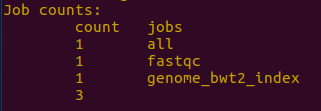
\includegraphics[width=6cm]{03_workflow/images/FAIR_ex1_o5_smk.png}
\end{center}
It is because the \verb|fastqc| rule is defined with a list of files and not for one unique file and because the \verb|fastqc| tool accepts both a unique file as well as a list of files.
\end{exampleblock}
\end{frame}
%-------------------------------------------
\begin{frame}[containsverbatim]
\frametitle{Running n individual jobs}
%-------------------------------------------
\begin{exampleblock}{Objective 6}
Thank to the \verb|all| rule, all expected files are designated. So we don't need to give the \verb|fastqc| rule a list anymore and we can replace it to manage only one file and all files one by one. We will gain in power in systems having more than one core.
\end{exampleblock}
\begin{exampleblock}{Hint}
Replace the \verb|expand()| function with a wildcard for one filename in the \verb|fastqc| rule.
\end{exampleblock}
\end{frame}
%-------------------------------------------
\begin{frame}[containsverbatim]
\frametitle{Solution}
%-------------------------------------------
\begin{exampleblock}{ex1$\_$o6.smk}
\begin{lstlisting}
rule fastqc:
  output:
    "FastQC/{sample}_fastqc.zip",
    "FastQC/{sample}_fastqc.html"
  input:
    "Data/{sample}.fastq.gz"
  shell: "fastqc --outdir FastQC/ {input}"
\end{lstlisting}
\end{exampleblock}
\begin{exampleblock}{Snakemake run}
\begin{lstlisting}[language=python]
snakemake -s ex1_o6.smk -R all fastqc
\end{lstlisting}
\end{exampleblock}
\end{frame}
%-------------------------------------------
\begin{frame}[containsverbatim]
\frametitle{Solution}
%-------------------------------------------

\begin{exampleblock}{Observe result}
Now Snakemake did many fastqc jobs:
\begin{center}
    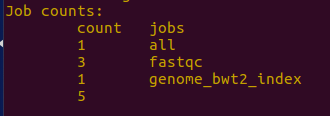
\includegraphics[width=6cm]{03_workflow/images/FAIR_ex1_o6_smk.png}
\end{center}
But what happens to the runtime displays on the screen?\\

To correct this, we will move the displays to a log file specific for each rule and each input file.
\end{exampleblock}
\end{frame}
%-------------------------------------------
\begin{frame}[containsverbatim]
\frametitle{Adding log file}
%-------------------------------------------
\begin{exampleblock}{Objective 7}
In Unix systems, the output of a command is usually sent to two separate streams: the normal output: to Standard Out (stdout also "\verb|>|" in shell), and error messages: to Standard Error (stderr, or "\verb|2>|" in shell). To integrate stderr into the same log file as the stdout can be use "\verb|&>|" instead of "\verb|>|": \\ 
shell: ...  \verb|&> {log}|", but use with care when output files are printed to stdout (as often in shell comands).\\
Redirect the stdout and stderr streams of the \verb|fastqc| and bowtie2-build commands. \\
\end{exampleblock}
\begin{exampleblock}{Hint}
For the \verb|bowtie2-build| and \verb|fastqc| rules, add the \verb|log:| directive with two variables (\verb|log1| and \verb|log2|) to redirect each streams.
\end{exampleblock}
\end{frame}
%-----------------------------------------------
\begin{frame}[containsverbatim]
\frametitle{Solution}
%-------------------------------------------
\begin{exampleblock}{ex1$\_$o7.smk}
\begin{lstlisting}[language=python]
# in rule genome_bwt2_index:
  log:
    log1="Logs/genome_bwt2_index.log1",
    log2="Logs/genome_bwt2_index.log2"
  shell: "bowtie2-build {input} Tmp/Otauri 1>{log.log1} 2>{log.log2}"
# in rule fastqc:
  log:
    log1="Logs/{sample}_fastqc.log1",
    log2="Logs/{sample}_fastqc.log2"
  shell: "fastqc --outdir FastQC/ {input} 1>{log.log1} 2>{log.log2}"
\end{lstlisting}
\end{exampleblock}
\begin{exampleblock}{Snakemake run}
\begin{lstlisting}[language=python]
rm -Rf FastQC/ Tmp/ Logs/; snakemake -s ex1_o7.smk
\end{lstlisting}
\end{exampleblock}
\end{frame}

%-------------------------------------------
\subsection[bash2snakemake]{From bash script to snakemake workflow}
%-------------------------------------------
\begin{frame}{How To?}
    \huge{From bash script to snakemake workflow}
\end{frame}
%-------------------------------------------
\begin{frame}[containsverbatim]
\frametitle{Snakemake point}
%-------------------------------------------
\begin{block}{So far, we've seen:}
\begin{itemize}
    \item the rule and the workflow concepts, the snakefile
    \item how rules are linked thank to input/output files and the first rule, the target rule
    \item how to generalize the inputs of a rule using wildcards on filenames (and the expand function)
    \item how to redirect stdout and sdterr streams (log)
\end{itemize}
\end{block}
\begin{block}{From now, we will seen:}
\begin{itemize}
    \item some snakemake options: to visualize the workflow diagram, use a dry-run option, etc
    \item adding a configuration file
    \item getting file names from the file system
    \item \alert{the container directive ???}
    \item \alert{how to run snakemake on cluster ???}
\end{itemize}
\end{block}
\end{frame}
%-------------------------------------------
\begin{frame}[containsverbatim]
\frametitle{Snakemake DAG visualization}
%-------------------------------------------
\begin{block}{}
Snakemake use Graphviz (\verb|dot| command) to create graphical visualisations, for the complete workflow (--dag) or for the rules dependencies (--rulegraph):
\begin{lstlisting}
snakemake --dag  | dot | display
snakemake --dag  | dot -Tpng > dag.png
\end{lstlisting}
\end{block}
\begin{center}
    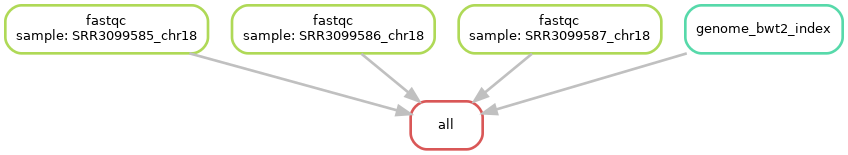
\includegraphics[width=12cm]{03_workflow/images/FAIR_ex1_o7_dag.png}\\
    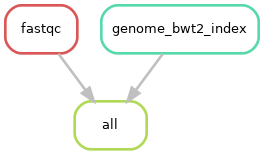
\includegraphics[width=3cm]{03_workflow/images/FAIR_ex1_o5_ruleG.png}
\end{center}
\end{frame}
%-------------------------------------------
\begin{frame}[containsverbatim]
\frametitle{Some Snakemake options}
%-------------------------------------------
\begin{block}{Running options}
\begin{itemize}
    \item automatically create HTML reports (\verb|--report report.html|) containing runtime statistics, a visualization of the workflow topology, used software and data provenance information
    \item dry-run, do not execute anything, display what would be done: \verb|-n --dryrun|
    \item print the executed shell command: \verb|-p --printshellcmds |
    \item print the reason for each rule execution: \verb|-r --reason|
    \item print a summary and status of rule: \verb|-D|
    \item limit the number of jobs in parallel: \verb|-j 1| (cores: \verb|--cores 1|)
\end{itemize}
\end{block}
\vfill
\href{https://snakemake.readthedocs.io/en/stable/executing/cli.html#all-option}{\textcolor{blue}{\underline{all Snakemake options}}}
\end{frame}
%-------------------------------------------
\begin{frame}[containsverbatim]
\frametitle{Some Snakemake options}
%-------------------------------------------
\begin{block}{Configuration file}
Use a configuration file to place all hard-coding values (paths, core numbers, parameters, etc):
\begin{itemize}
    \item can be write both in yml or in json
    \item add Snakemake option: \verb|--configfile file.yml| or add \verb|configfile: file.yml| at the beginning of the snakefile
    \item Snakefile call of defined items: \verb|config["item1"]| in input/output directive and \verb|{config[item1]}| in shell directive
\end{itemize}
\end{block}
\end{frame}
%-------------------------------------------
\begin{frame}[containsverbatim]
\frametitle{File names from the file system}
%-------------------------------------------
To infer the identifiers (IDs) from present files in a directory, use the inbuilt \verb|glob_wildcards| function:
\begin{block}{Ex. of the glob$\_$wilcards function}
\begin{lstlisting}
IDs, = glob_wildcards("thedir/{id}.fastq")
\end{lstlisting}
\end{block}
\verb|glob_wildcards()| matches the given pattern against the files present in the file system and thereby infers the values for all wildcards in the pattern, \verb|{id}| here. 
\vfill
Don't forget the coma after the name (left hand side, \verb|IDs| here).
\end{frame}
%-------------------------------------------
\begin{frame}[containsverbatim]
\frametitle{Conda environment}
%-------------------------------------------
\begin{block}{}
In the practical exercise we will have one conda environment for executing the whole Snakemake workflow. \\
Snakemake also supports using explicit conda environments on a per-rule basis:
\begin{itemize}
    \item add the \verb|conda: rule-specific-env.yml| directive in the rule definition 
    \item run Snakemake with the \verb|--use-conda| option 
\end{itemize}
The specified environment will be created and activated on the fly by Snakemake and the rule will then be run in the conda environment.
\end{block}
\end{frame}
%-------------------------------------------
\begin{frame}[containsverbatim]
\frametitle{Container directive}
%-------------------------------------------
\end{frame}
%-------------------------------------------
\begin{frame}[containsverbatim]
\frametitle{Cluster option}
%-------------------------------------------

\end{frame}


%-------------------------------------------
\subsection[SnakemakeEx2]{Exercise 2: finalize the RNAseq analysis workflow}
%-------------------------------------------
\begin{frame}{}
    \huge{Exercise 2: workflow of the RNAseq analysis}
\end{frame}
%-------------------------------------------
\begin{frame}{RNAseq analysis}
%\againframe<2>{RNAseqWF_diapo}
%-------------------------------------------
\begin{block}{Analysis workflow}
    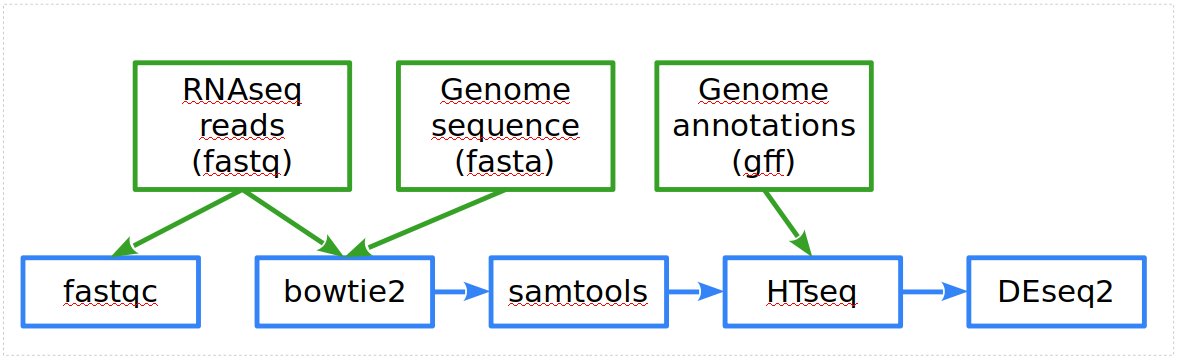
\includegraphics[width=12cm]{01_introduction/images/FAIR_RNAseq_WF.png}\\
green=input, blue=tool
\end{block}
\footnotesize{
\begin{description}
    \item[fastqc] control quality of the input reads
    \item[bowtie2] reads mapping on the genome sequence
    \item[samtools] mapped reads selection $\&$ formatting
    \item[HTseq] count table of mapped reads on genes (annotations)
    \item[DEseq2] statistical analysis: genes list having differential expression
\end{description}
}
\end{frame}
%-------------------------------------------
\begin{frame}[containsverbatim]
\frametitle{Data and command line}
%-------------------------------------------
\begin{exampleblock}{Data}
-g genome sequence acces (including extention .fna, .fasta)\\
-a genome annotation acces (inluding extention .gff)\\
-d RNAseq sample prefix\\
next args: RNAseq sample prefix, no .fastq.gz extention
\end{exampleblock}
\begin{exampleblock}{Bash command line}
\begin{lstlisting}
FAIR_initial_script.sh -g ../O.tauri_genome.fna -a ../O.tauri_annotation.gff -d ../ SRR3099585_chr18 S*86_chr18 S*87_chr18 S*97_chr18 S*98_chr18 S*99_chr18
\end{lstlisting}
\end{exampleblock}
\begin{exampleblock}{Script in 3 main blocks}
\begin{lstlisting}
1) while getops do ... done   
2) for sample in $* ; do ... done   
3) creation of the result file, counts.txt, with paste, awk, and sed bash commands
\end{lstlisting}
\end{exampleblock}
\end{frame}
%-------------------------------------------
\begin{frame}[containsverbatim]
\frametitle{Complete bash script, 1/3}
%-------------------------------------------
\begin{exampleblock}{getops block}
\begin{lstlisting}
while getopts g:a:d: flag do
        case $flag in
            g)  genome=$OPTARG
                echo genome is $genome ;;
            a)  annots=$OPTARG
                echo annotation is $annots ;;
            d)  rnadir=$OPTARG
                echo RNAseq path is $rnadir ;;
            :)  echo "L'option $OPTARG requiert un argument"
                exit 1 ;;
            \?) echo "$OPTARG : option invalide"
                exit 1 ;;
        esac
   done
shift $(( OPTIND - 1 ))  # shift past the last flag or argument
echo samples are $*
\end{lstlisting}
\end{exampleblock}
\end{frame}
%-------------------------------------------
\begin{frame}[containsverbatim]
\frametitle{Complete bash script, 2/3}
%-------------------------------------------
\begin{exampleblock}{for block}
\begin{lstlisting}
nbs=0;
for sample in $* ; do 
   nbs=$(expr ${nbs} + 1)
   echo traitement of sample ${sample}
   # --------- quality control of reads
   if [ ! -d FastQC ]; then
       mkdir FastQC
   fi
   fastqc --outdir FastQC ${rnadir}${sample}.fastq.gz > FastQC/${sample}.log 2>&1
   #---------- reads mapping
   if [ ! -d Bwt2_index ]; then
       mkdir Bwt2_index
       bowtie2-build ${genome} Bwt2_index/tauri > Bwt2_index/Bwt2_index.log 2>&1
   fi
\end{lstlisting}
\end{exampleblock}
\end{frame}
%-------------------------------------------
\begin{frame}[containsverbatim]
\frametitle{Complete bash script, 3/3}
%-------------------------------------------
\begin{exampleblock}{for block, continuation}
\begin{lstlisting}
   bowtie2 -x Bwt2_index/tauri -U ${rnadir}${sample}.fastq.gz -S ${sample}.sam > ${sample}_bowtie2.log 2>&1
   #---------- selection and format modification
   samtools view -b ${sample}.sam -o ${sample}.bam
   samtools sort ${sample}.bam -o ${sample}_sort.bam
   samtools index ${sample}_sort.bam
   #---------- counting of mapped reads by gene
   featureCounts -t gene -g ID -a ${annots} -s 2 -o ${sample}_ftc.txt ${sample}_sort.bam > ${sample}_ftc.log 2>&1
done
\end{lstlisting}
\end{exampleblock}
\begin{exampleblock}{Count table block}
\begin{lstlisting}
paste *_ftc.txt > ftc_tmp.txt
awk -v nb=${nbs} -v col=7 'BEGIN{FS="\t"}{ctmp=$1; for(i=col;i<=nb*col;i=i+col){count=sprintf("%s\t%s",ctmp,$i);ctmp=count};print count}' ftc_tmp.txt | sed 1d > counts.txt
\end{lstlisting}
\end{exampleblock}
\end{frame}
%-------------------------------------------
\begin{frame}[containsverbatim]
\frametitle{Exercise 2}
%-------------------------------------------
Continue the snakefile of the previous exercise in order to replace the bash script. \\
We will:
\begin{exampleblock}{Objectives}
\begin{itemize}
    \item add a configuration file
    \item use a builtin snakemake function to get filenames of the input RNAseq data
    \item add rules to replace the mapping, formatting, counting, and counts aggregating steps of the bash script
\end{itemize}
\end{exampleblock}
\begin{exampleblock}{ex2$\_$o1.smk}
\begin{lstlisting}
cp ex1_o7.smk ex2_o1.smk
\end{lstlisting}
\end{exampleblock}
\end{frame}
%-------------------------------------------
\begin{frame}[containsverbatim]
\frametitle{getops block}
%-------------------------------------------
\begin{exampleblock}{Shell script}
\begin{lstlisting}
while getopts g:a:d: flag do
        case $flag in
            g)  genome=$OPTARG 
            ...
\end{lstlisting}
\end{exampleblock}
We will use a configuration file:
\begin{exampleblock}{Objective 1}
Add a configuration file, named \verb|RNAseq.yml|, containing both the genome sequence and the annotation files manes, and the access to the Data directory. \\
In the snakefile, change the configured variables (ex. replace \verb|Data/| and \verb|genome| by their \verb|config[]| values). The Python strings concatenation is \verb|+|\\
Then, run snakemake with the \verb|--configfile| option.
\end{exampleblock}
\end{frame}
%-------------------------------------------
\begin{frame}[containsverbatim]
\frametitle{Adding a configuration file}
%-------------------------------------------
\begin{exampleblock}{ex2$\_$o1.yml}
\begin{lstlisting}
genome:
  O.tauri.fna
annots:
  O.tauri.gff
dataDir:
  Data/
\end{lstlisting}
\end{exampleblock}
\begin{exampleblock}{ex2$\_$o1.smk: "Data/..." in inputs replaced by a config call:}
\begin{lstlisting}
rule genome_bwt2_index:   config["dataDir"]+config["genome"]
rule fastqc:   config["dataDir"]+"{sample}.fastq.gz"
\end{lstlisting}
\end{exampleblock}
\begin{exampleblock}{snakemake run:}
\begin{lstlisting}
rm -Rf FastQC/ Result/ Tmp/ Logs/ ; snakemake -s ex2_o1.smk --configfile ex2_o1.yml
\end{lstlisting}
\end{exampleblock}
\end{frame}
%-------------------------------------------
\begin{frame}[containsverbatim]
\frametitle{for block}
%-------------------------------------------
\begin{exampleblock}{Shell script}
\begin{lstlisting}
nbs=0;
for sample in $* ; do 
   ...
done
\end{lstlisting}
\end{exampleblock}
To manage all *.fastq.gz files in a directory, use the \verb|glob_wilcards()| function. In \verb|ex2_o2.smk|, replace the SAMPLES definition by:
\begin{exampleblock}{ex2$\_$o2.smk}
\begin{lstlisting}
SAMPLES, = glob_wildcards(config["dataDir"]+"{sample}.fastq.gz")
\end{lstlisting}
\end{exampleblock}
and run snakemake.
\end{frame}
%-------------------------------------------
\begin{frame}[containsverbatim]
\frametitle{Quality control, fastqc}
%-------------------------------------------
\begin{exampleblock}{}
\begin{lstlisting}
if [ ! -d FastQC ]; then
   mkdir FastQC
fi
fastqc --outdir FastQC ${sample}.fastq.gz > FastQC/${sample}.log 2>&1
\end{lstlisting}
\end{exampleblock}
No more need to test the existence of a directory, it is created as needed.
\begin{exampleblock}{rule fastqc:}
This rule is already present in the snakefile
\end{exampleblock}
\end{frame}
%-------------------------------------------
\begin{frame}[containsverbatim]
\frametitle{Reads mapping, bowtie2}
%-------------------------------------------
\begin{exampleblock}{}
\begin{lstlisting}
if [ ! -d Bwt2_index ]; then
   mkdir Bwt2_index
   bowtie2-build ${genome} Bwt2_index/tauri > Bwt2_index/Bwt2_index.log 2>&1
fi
bowtie2 -x Bwt2_index/tauri -U ${sample}.fastq.gz -S ${sample}.sam > ${sample}_bowtie2.log 2>&1
\end{lstlisting}
\end{exampleblock}
2 rules: \verb|genome_bwt2_index| (cf. previous ex.) and \verb|bwt2_mapping|
\begin{exampleblock}{ex2$\_$o3.smk, rule bwt2$\_$mapping (no run):}
\begin{lstlisting}
  output: "results/{sample}.sam"
  input: config["dataDir"]+"{sample}.fastq.gz",
         expand("Tmp/Otauri.{ext}.bt2", ext=BIDX)
  log: "Logs/{sample}_bwt2_mapping.log"
  shell: "bowtie2 -x Tmp/Otauri -U {input[0]} -S {output} 2> {log} "
\end{lstlisting}
\end{exampleblock}
\end{frame}
%-------------------------------------------
\begin{frame}[containsverbatim]
\frametitle{Reads mapping, bowtie2}
%-------------------------------------------
\begin{exampleblock}{Why some troubles?}
The snakemake launch probably didn't do what was expected. 
What have we forgotten? \\
We added a new rule to a snakemake but we didn't manage the rule tree, their is no input-output link to include the new rule to the workflow.\\
We will do that by completing the input directive of the target rule (caution to respect the Python "list" structure, coma-separated).
\end{exampleblock}
\begin{exampleblock}{ex2$\_$o2.smk, target rule:}
\begin{lstlisting}
rule all:
  input:
    expand("FastQC/{sample}_fastqc.html", sample=SAMPLES),
    expand("Tmp/Otauri.{ext}.bt2", ext=BIDX),
    expand("Tmp/{sample}.sam", sample=SAMPLES)
\end{lstlisting}
\end{exampleblock}
\end{frame}
%-------------------------------------------
\begin{frame}[containsverbatim]
\frametitle{samtools}
%-------------------------------------------
\begin{exampleblock}{Shell script}
\begin{lstlisting}
samtools sort -O bam -o ${sample}_sort.bam ${sample}.sam
samtools index ${sample}_sort.bam
\end{lstlisting}
\end{exampleblock}
\begin{exampleblock}{ex2$\_$o4.smk, rule sam2bam$\_$sort (no run):}
\begin{lstlisting}
  output:
    bam="Result/{sample}_sort.bam",
    bai="Result/{sample}_sort.bam.bai"
  input: "Tmp/{sample}.sam"
  log:
    sort="Logs/{sample}_sam2bam_sort.log",
    index="Logs/{sample}_bam2bai.log"
  shell: 
    "samtools sort -O bam -o {output.bam} {input} 2> {log.sort} ;"
    "samtools index {output.bam} 2> {log.index}"
\end{lstlisting}
\end{exampleblock}
\end{frame}
%-------------------------------------------
\begin{frame}[containsverbatim]
\frametitle{FeatureCount}
%-------------------------------------------
\begin{exampleblock}{Shell script}
\begin{lstlisting}
featureCounts -t gene -g ID -a ${annots} -s 2 -o ${sample}_ftc.txt ${sample}_sort.bam > ${sample}_ftc.log 2>&1
\end{lstlisting}
\end{exampleblock}
\begin{exampleblock}{ex2$\_$o5.smk, rule counting (params; no run):}
\begin{lstlisting}
  output: "Tmp/{sample}_ftc.txt"
  input:
    bam="Result/{sample}_sort.bam",
    annot=config["dataDir"]+config["annots"]
  params: t="gene", g="ID", s="2"
  log: "Logs/{sample}_counts.log"
  shell: "featureCounts -t {params.t} -g {params.g} -a {input.annot} -s {params.s} -o {output} {input.bam} &> {log}"
\end{lstlisting}
\end{exampleblock}
\end{frame}
%-------------------------------------------
\begin{frame}[containsverbatim]
\frametitle{Counts matrix creation}
%-------------------------------------------
\begin{exampleblock}{Shell script}
\begin{lstlisting}
paste *_ftc.txt > counts_tmp.txt
awk -v nb=${nb_sample} 'BEGIN{FS="\t"}{count_tmp=$1; for(i=7;i<=nb*7;i=i+7){count=sprintf("%s\t%s",count_tmp,$i);count_tmp=count};print count}' counts_tmp.txt | sed 1d > counts.txt
\end{lstlisting}
\end{exampleblock}
\begin{exampleblock}{Hint}
Create 2 rules to manage some files aggregation to one result file:
\begin{itemize}
    \item rule \verb|extract_counts|: extract geneID and counts in individual files
    \item rule \verb|matrix_counts|: paste these files
\end{itemize} 
\end{exampleblock}
\end{frame}
%-------------------------------------------
\begin{frame}[containsverbatim]
\frametitle{Counts matrix creation}
%-------------------------------------------
\begin{exampleblock}{ex2$\_$o6.smk (2 rules, shell 3", copy, run):}
\begin{lstlisting}
rule matrix_counts:
  output: "Result/counts_matrix.txt"
  input: countfile=expand("Tmp/{sample}_ftc7.txt", sample=SAMPLES), geneID=expand("Tmp/{sample}_ftc1.txt", sample=SAMPLES)
  log: "Logs/matrix_counts.log"
  shell: """cp {input.geneID[0]} Tmp/ftc_geneID.txt > {log} ; paste Tmp/ftc_geneID.txt {input.countfile} > {output} > {log}"""

rule extract_counts:
  output: col7="Tmp/{sample}_ftc7.txt",
          col1="Tmp/{sample}_ftc1.txt"
  input: "Tmp/{sample}_ftc.txt"
  log: "Logs/{sample}_extract_counts.log"
  shell: """cut -f 7 {input} | sed 1d > {output.col7} > {log} ; cut -f 1 {input} | sed 1d > {output.col1} """
\end{lstlisting}
\end{exampleblock}
\end{frame}
%-------------------------------------------
\begin{frame}[containsverbatim]
\frametitle{DESeq2}
%-------------------------------------------
The DESeq2 step is the statistical analysis. From the count matrix, the statistical analysis is managed by a non parallelizable R script, DESeq2.
\vfill
So, up to date, the workflow is complete and the only thing left is this DESeq2 statistical analysis. We will see this analysis through the notebooks session.
\end{frame}
%-------------------------------------------
\begin{frame}[containsverbatim]
\frametitle{Last challenge}
%-------------------------------------------
\begin{exampleblock}{}
Clean, delete and re-run !
\begin{lstlisting}
cp ex2_o8.smk RNAseq_analysis.smk
cp ex2_o1.yml RNAseq_analysis_smkEnv.yml
rm -Rf FastQC/ Results/ Logs/ Tmp/ 
snakemake -s  RNAseq_analysis.smk --configfile RNAseq_analysis_smkEnv.yml
\end{lstlisting}
\end{exampleblock}
\end{frame}
%-------------------------------------------
\begin{frame}[containsverbatim]
\frametitle{Bonus}
%-------------------------------------------
\begin{exampleblock}{Add a help rule}
\url{https://lachlandeer.github.io/snakemake-econ-r-tutorial/self-documenting-help.html#a-help-rule}
\end{exampleblock}
\end{frame}


%-------------------------------------------
\begin{frame}{Snakemake conclusion}
%-------------------------------------------
\begin{block}{Power gain}
We have transposed the shell srcipt to a snakefile associated to a configuration file. This solution will be more powerful when we apply it in a High Performance Computing environment like the IFB cluster.
\end{block}
\begin{block}{Reprodicibility issue}
In terms of reproducibility, we have to focus on the tools environment.
\end{block}
\end{frame}
%-------------------------------------------
\begin{frame}{Ressources}
\begin{description}
    \item [Official documentation] https://snakemake.readthedocs.io/en/stable/
    \item [Johannes Koëster publication] https://doi.org/10.1093/bioinformatics/bts480
    \item [bioinfo-fr.net]  https://bioinfo-fr.net (+search snakemake)
    \item [begining of a gitbook] https://endrebak.gitbooks.io/the-snakemake-book
\end{description}
    
\end{frame}


\end{document}